%!TEX TS-program = xelatex
%!TEX encoding = UTF-8 Unicode

\documentclass[11pt,tikz,border=1]{standalone}
\usetikzlibrary{calc,positioning}

\usepackage[default,mdseries=Light,bfseries=Medium,path=../fonts]{cjkfonts}
% file: westernfonts.tex

\newfontfamily\SourceCodePro{SourceCodePro}[
  UprightFont=*-Light,
  BoldFont=*-Medium,
  ItalicFont=*-LightIt,
  BoldItalicFont=*-MediumIt]

\newfontfamily\SourceSerifPro{SourceSerifPro}[
  UprightFont=*-Light,
  BoldFont=*-Semibold]

\newcommand{\serif}[0]{\SourceSerifPro}
 
\setmonofont{SourceCodePro}[
  UprightFont=*-Light,
  BoldFont=*-Medium,
  ItalicFont=*-LightIt,
  BoldItalicFont=*-MediumIt]


\begin{document}
  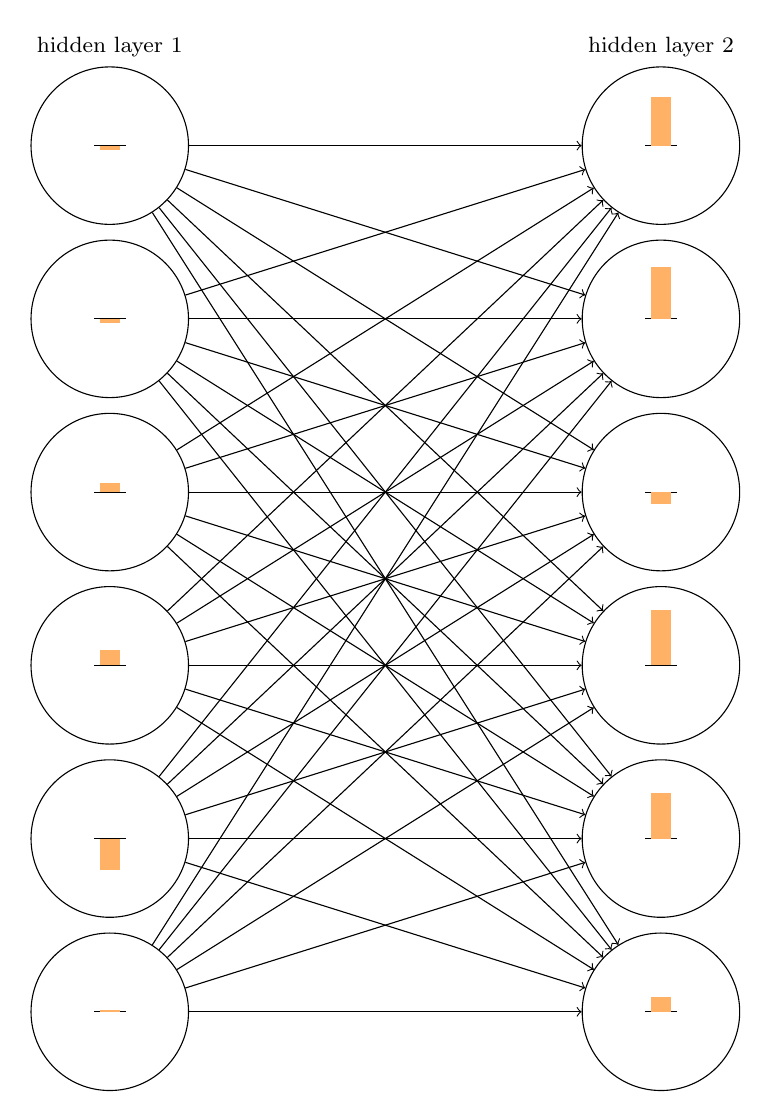
\begin{tikzpicture}[
    neuron/.style={circle,draw,inner sep=0pt,minimum size=20mm},
    font=\footnotesize
    ]

    \foreach \x in {0,...,5} {
      \node(l\x) [neuron] at (0, 2.2 * \x) {};
      \node(r\x) [neuron] at (7, 2.2 * \x) {};
    }

    \node [above] at (l5.north) {\RobotoLight hidden layer 1};
    \node [above] at (r5.north) {\RobotoLight hidden layer 2};

    \foreach \x in {0,...,5} 
      \foreach \y in {0,...,5}
        \draw[->] (l\x) to (r\y);

    \foreach \x in {0,...,5} {
      \coordinate (c) at (l\x.center);
      \draw ($(c)+(-2mm,0)$) -- ($(c)+(2mm,0)$);
      \coordinate (c) at (r\x.center);
      \draw ($(c)+(-2mm,0)$) -- ($(c)+(2mm,0)$);
    }
    
    \coordinate (c) at (l5.center);
    \fill[fill=orange!60] ($(c)+(-1.25mm,0)$) rectangle ($(c)+(1.25mm,-0.003970677333144113mm * 150)$);
    \coordinate (c) at (l4.center);
    \fill[fill=orange!60] ($(c)+(-1.25mm,0)$) rectangle ($(c)+(1.25mm,-0.0031684316985881185mm * 150)$);
    \coordinate (c) at (l3.center);
    \fill[fill=orange!60] ($(c)+(-1.25mm,0)$) rectangle ($(c)+(1.25mm,0.008103235909196014mm * 150)$);
    \coordinate (c) at (l2.center);
    \fill[fill=orange!60] ($(c)+(-1.25mm,0)$) rectangle ($(c)+(1.25mm,0.012598010584130365mm * 150)$);
    \coordinate (c) at (l1.center);
    \fill[fill=orange!60] ($(c)+(-1.25mm,0)$) rectangle ($(c)+(1.25mm,-0.026465907331998335mm * 150)$);
    \coordinate (c) at (l0.center);
    \fill[fill=orange!60] ($(c)+(-1.25mm,0)$) rectangle ($(c)+(1.25mm,0.0017583319323150341mm * 150)$);

    \coordinate (c) at (r5.center);
    \fill[fill=orange!60] ($(c)+(-1.25mm,0)$) rectangle ($(c)+(1.25mm,0.04152906589960523mm * 150)$);
    \coordinate (c) at (r4.center);
    \fill[fill=orange!60] ($(c)+(-1.25mm,0)$) rectangle ($(c)+(1.25mm,0.044025552524932406mm * 150)$);
    \coordinate (c) at (r3.center);
    \fill[fill=orange!60] ($(c)+(-1.25mm,0)$) rectangle ($(c)+(1.25mm,-0.009669682279354514mm * 150)$);
    \coordinate (c) at (r2.center);
    \fill[fill=orange!60] ($(c)+(-1.25mm,0)$) rectangle ($(c)+(1.25mm,0.046736871369353235mm * 150)$);
    \coordinate (c) at (r1.center);
    \fill[fill=orange!60] ($(c)+(-1.25mm,0)$) rectangle ($(c)+(1.25mm,0.03877302528270452mm * 150)$);
    \coordinate (c) at (r0.center);
    \fill[fill=orange!60] ($(c)+(-1.25mm,0)$) rectangle ($(c)+(1.25mm,0.012336459551975156mm * 150)$);


  \end{tikzpicture}
\end{document}
